\documentclass[3_juin_2023.tex]{subfiles}
\begin{document}
\pagestyle{empty}
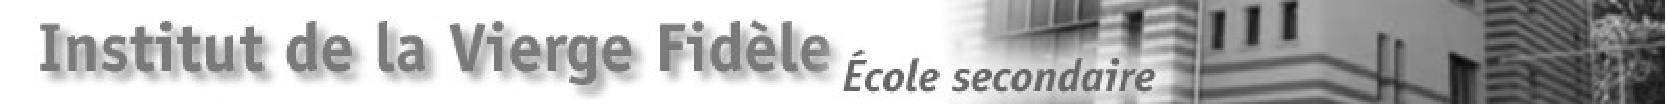
\includegraphics[width=\linewidth]{img/entete.pdf}
\vspace{\smallskipamount}
\begin{tblr}{%
        hline{1,3,5,9,10},
        vline{1,4},
        colspec={XXX},%
        cell{1}{1} = {r=1, c=3}{c,font=\bfseries\Huge},%
        cell{2}{1}= {r=1, c=3}{c,font=\bfseries\Large},%
        cell{3}{1}={r=1,c=2}{l},
        cell{4}{1}={r=1,c=2}{l},
        cell{5}{1}={r=1,c=2}{l},
        cell{5}{3}={r=2,c=1}{c},
        cell{6}{1}={r=1,c=2}{l},%
        cell{7}{1}={r=1,c=3}{l},%
        cell{8}{1}={r=1,c=3}{l},%
        row{9}={c},
        rowsep=1ex%
    }%
    % cell1
    Mathématiques                                                   &   &                                                   \\
    % cell2
    Partie 2                                                       &   &                                                   \\
    % cell3
    Nom :                                                           &   & Classe :                                          \\
    % cell4
    Prénom :                                                        &   & Numéro :                                          \\
    % cell5
    Professeurs :  Baudoin, Debroux, Regout                          &   & \\
    % cell6
    Date et heure: Lundi 19 juin 2023 de 10 h 45 à 12 h 50          &   &                                                   \\
    % cell7
    Matériel autorisé : calculatrice                                &   &                                                   \\
    % cell8
    Matériel à distribuer : feuille à en-tête, feuille de brouillon &   &                                                   \\
    % % cell9
    % C1 : \qquad/\TotalExerciseTypeGoal{connaitre}{points}{}{}
    %                                                                 &
    % C2 : \qquad/\TotalExerciseTypeGoal{appliquer}{points}{}{}
    %                                                                 &
    % C3 : \qquad/\TotalExerciseTypeGoal{transferer}{points}{}{}                                                              \\
\end{tblr}%
\vspace{\smallskipamount}
\begin{scriptsize}%
    Rue de linthout, 30 - 1030 Bruxelles%
\end{scriptsize}%
\par%
\minisec{Quelques consignes}
\begin{itemize}
    \item Rendre une copie soignée et aérée.
    \item Respecter les conventions mathématiques et les notations.
    \item Détailler tous ses raisonnements, la réponse seule ne suffit pas.
    \item Pour les problèmes, n'oubliez pas de formuler la réponse finale  avec une phrase complète.
    \item Arrondir les réponses finales (pas d'arrondis sur les réponses intermédiaires) au centième près.
\end{itemize}
\faIcon{exclamation-triangle} Tout manquement entraînera une perte de points, soyez vigilant lors de la relecture.
\vfill
\begin{flushright}
    Bon travail !
\end{flushright}
\cleardoublepage
\pagestyle{plain}
\setcounter{page}{1}
%====
% C1
%====
%%%%%%%%%%%%%%%%%%%%%%%%%%%%%%%%%%%%%%%
% EXERCICE
\begin{connaitre}[points=3]
    Détermine la ou les bonnes réponses. Si tu oublies des bonnes réponses ou que tu coches des mauvaises réponses, tu n'obtiens aucun point pour l'énoncé.
    \begin{enumerate}
        % \item \parbox[t]{.6\linewidth}{Dans le cercle ci-contre de centre $O$, les points $A,\ B,\ C,\ D$ et $E$ appartiennent au cercle. Les points $B,\ O$ et $C$ sont alignés.}
        %       \hfill
        %       \begin{tikzpicture}[baseline=(current bounding box.east), scale=2]
    \tkzDefPoint(0,0){O}
    \tkzDefPoint(30:1){A}
    \tkzDefPoint(180:1){B}
    \tkzDefPoint(0:1){C}
    \tkzDefPoint(-97:1){D}
    \tkzDefPoint(100:1){E}
    \tkzDrawCircle(O,A)
    \tkzDrawPoints(A,B,C,D,E,O)
    \tkzLabelPoints[above right](A)
    \tkzLabelPoints[left](B)
    \tkzLabelPoints[below right](C)
    \tkzLabelPoints[below](D)
    \tkzLabelPoints[above](E)
    \tkzLabelPoints[below](O)
\end{tikzpicture}
        %       \begin{QCM}(2)
        %           \choice $|\widehat{BAC}|=\ang{90}$
        %           \choice $|\widehat{ADB}| = 2|\widehat{BAD}|$
        %           \choice $|\widehat{BOD}| = \ang{90}$
        %           \choice $|\widehat{BED}| = |\widehat{BAD}|$
        %       \end{QCM}
        \item Dans un triangle $ABC$ rectangle en $A$ \dots
              \begin{QCM}
                  \choice $\sin^2\widehat{B} + \cos^2\widehat{B}=1$
                  \choice $\tan\widehat{C} = \dfrac{\cos\widehat{C}}{\sin\widehat{C}}$
                  \choice $|BC|^2 = |AB|^2 + |AC|^2$
                  \choice $\cos\widehat{C}=\dfrac{|AB|}{|BC|}$
              \end{QCM}
        \item Quels sont les proportions exactes si $CB\sslash DE$ ? \begin{tikzpicture}[baseline=(current bounding box.east)]
    \tikzmath{
        \myangle = 30;
        \a = 1;
        \b = 1.5;
        \k = 2;
    }
    \tkzDefPoint(0,0){A}
    \tkzDefPoint(\a,0){B}
    \tkzDefPoint(\myangle:\b){C}
    \tkzDefPointBy[homothety=center A ratio \k](B)
    \tkzGetPoint{D}
    \tkzDefLine[parallel= through D](B,C)
    \tkzInterLL(A,C)(D,tkzPointResult)
    \tkzGetPoint{E}

    \tkzLabelPoints[below](A,B,D)
    \tkzLabelPoints[above](C,E)
    % \tkzDrawPoints(A,B,C,D,E)

    \tkzDrawPolygons(E,D,A B,A,C)
    
\end{tikzpicture}
              \begin{QCM}(4)
                  \choice $\dfrac{|AC|}{|AB|}=\dfrac{|AE|}{|AD|}$
                  \choice $\dfrac{|AB|}{|BD|}=\dfrac{|AC|}{|AE|}$
                  \choice*(2) $|AC|\cdot |AD| = |AB| \cdot |AE|$
              \end{QCM}
        \item Si $ABC$ et $DEF$ sont deux triangles semblables tels que $DEF$ est l'image de $ABC$ par une similitude de coefficient $k=8$ alors \dots
              \begin{QCM}(5)
                  \choice*(2) Le périmètre de $ABC$ est supérieur à celui de $DEF$.
                  \choice $\dfrac{|DE|}{|AB|}=8$
                  \choice*(2) L'amplitude des angles de $ABC$ sont 8 fois plus petit que ceux de $DEF$.
              \end{QCM}
              % \item Deux triangles semblables \dots
              %       \begin{QCM}(3)
              %           \choice ont toujours la même aire.
              %           \choice ont des côtés homologues de longueurs proportionnelles.
              %           \choice ont des angles de même amplitude.
              %       \end{QCM}
              % \item Si $ABC$ est un triangle rectangle en $A$, alors \dots
              %       \begin{QCM}(3)
              %           \choice $\sin\widehat{C} = \dfrac{|AB|}{|BC|}$
              %           \choice $\cos\widehat{C} = \dfrac{|AB|}{|BC|}$
              %           \choice $\tan\widehat{B} = \dfrac{|AC|}{|ABC|}$
              %       \end{QCM}
    \end{enumerate}
\end{connaitre}
% SOLUTION
\begin{solution}
    Évaluations :
    \begin{itemize}
        \item Les bonnes réponses sont cochées et aucune mauvaise réponse n'est cochée \hfill 1
    \end{itemize}
    \begin{enumerate}
        \item
              \begin{QCM}(2)
                  \choice[\faCheckSquare]
                  $|\widehat{BAC}|=\ang{90}$

                  \choice
                  $|\widehat{ADB}| = 2|\widehat{BAD}|$

                  \choice
                  $|\widehat{BOD}| = \ang{90}$

                  \choice[\faCheckSquare]
                  $|\widehat{BED}| = |\widehat{BAD}|$
              \end{QCM}
        \item
              \begin{QCM}
                  \choice
                  [\faCheckSquare] $\sin^2\widehat{B} + \cos^2\widehat{B}=1$

                  \choice
                  $\tan\widehat{C} = \dfrac{\cos\widehat{C}}{\sin\widehat{C}}$

                  \choice
                  [\faCheckSquare] $|BC|^2 = |AB|^2 + |AC|^2$

                  \choice
                  $\cos\widehat{C}=\dfrac{|AB|}{|BC|}$
              \end{QCM}
        \item
              \begin{QCM}(4)
                  \choice[\faCheckSquare]
                  $\dfrac{|AC|}{|AB|}=\dfrac{|AE|}{|AD|}$

                  \choice
                  $\dfrac{|AB|}{|BD|}=\dfrac{|AC|}{|AE|}$

                  \choice*(2)[\faCheckSquare]
                  $|AC|\cdot |AD| = |AB| \cdot |AE|$
              \end{QCM}
        \item
              \begin{QCM}(5)
                  \choice*(2)
                  Le périmètre de $ABC$ est supérieur à celui de $DEF$.

                  \choice[\faCheckSquare]
                  $\dfrac{|DE|}{|AB|}=8$

                  \choice*(2)
                  L'amplitude des angles de $ABC$ sont 8 fois plus petit que ceux de $DEF$.
              \end{QCM}
    \end{enumerate}
\end{solution}
%====
% C2
%====
\begin{appliquer}[points=2]
    Résous le système d'équations ci-dessous.
    \[\left\{\begin{aligned}
            -3x+y & = 2 \\
            2x+y  & =-3
        \end{aligned}\right.\]
\end{appliquer}
% SOLUTION
\begin{solution}

\end{solution}

\begin{appliquer}[points=5]
    Effectue les opérations ci-dessous. Simplifie au maximum ta réponse finale et n'oublie pas les conditions d'existence.
    \begin{enumerate}[cols=2]
        \item %3 pts
              $\dfrac{x-1}{x^2-4} + \dfrac{3}{x+2}$
        \item %2 pts
              $\dfrac{x+1}{x-2}\cdot\dfrac{x^2-4x+4}{x}$
    \end{enumerate}
\end{appliquer}
% SOLUTION
\begin{solution}
    \begin{enumerate}
        \item
              Évaluation :
              \begin{itemize}
                  \item Factorisation \hfill 1
                  \item Condition d'existence \hfill 1
                  \item Simplification \hfill 0,5
              \end{itemize}
              $\begin{aligned}[t]
                      \dfrac{4}{x(3+x)}\div\dfrac{x-3}{(x-3)(x+3)} & = \dfrac{4}{3+x}\cdot (x+3)
                      \qquad\text{ C.E. : }x\ne 3\text{ et } x\ne -3                             \\
                                                                   & = 4
                  \end{aligned}$
        \item
              Évaluation :
              \begin{itemize}
                  \item Factorisation \hfill 1
                  \item Condition d'existence \hfill 1
                  \item Simplification \hfill 0,5
              \end{itemize}
              $\begin{aligned}[t]
                      \dfrac{x+1}{x-2} \cdot \dfrac{(x-2)^2}{x}
                       & = \dfrac{(x+1)(x-2)}{x}\qquad\text{C.E. : }x\ne 2 \text{ et } x \ne 0 \\
                  \end{aligned}$
    \end{enumerate}
\end{solution}
\newpage
\begin{appliquer}[points=6]
    Pour chaque figure ci-dessous, détermine les grandeurs manquantes en mobilisant la théorie adéquate. Note tous tes raisonnements et arrondis tes réponses au dixième si nécessaire (une réponse sous forme de fraction ou de racine carrée est préférée).

    \begin{tasks}[after-item-skip=2cm](3)
        \task
        $|AC| = ?$ et $|\widehat{C}|=?$
        \begin{center}
            \includegraphics[width=\linewidth]{tikz/c2_triangle_rectangle_001.tikz}
        \end{center}

        \task
        $|AC|=?$ et $|BC|=?$
        \begin{center}
            \includegraphics[width=\linewidth]{tikz/c2_trigonometrie1.tikz}
        \end{center}

        \task
        $DE \sslash BC$\\$|AD|=?$ et $|BC|=?$
        \begin{center}
            \includegraphics[width=\linewidth]{tikz/c2_thales2.tikz}
        \end{center}
    \end{tasks}
\end{appliquer}
% SOLUTION
\begin{solution}
    Évaluations :
    \begin{itemize}
        \item Le raisonnement est correcte et rigoureux\hfill 0,5
        \item La réponse est correcte \hfill 0,5
    \end{itemize}
    \begin{tasks}
        \task
        Comme le triangle $ABC$ est rectangle en $B$,
        \begin{itemize}
            \item
                  $
                      \begin{aligned}[t]
                          |AC|^2 & = |BC|^2 + |AB|^2                                            \\
                          |AC|   & = \sqrt{|BC|^2 + |AB|^2}                                     \\
                          |AC|   & = \sqrt{\left(\sqrt{32}\right)^2 + \left(\sqrt{17}\right)^2} \\
                          |AC|   & = \sqrt{49}                                                  \\
                          |AC|   & = 7
                      \end{aligned}
                  $
            \item
                  $
                      \begin{aligned}[t]
                          |\widehat{C}| & = \arctan\left(\dfrac{\sqrt{17}}{\sqrt{32}}\right) \\
                          |\widehat{C}| & = \ang{36,1}
                      \end{aligned}
                  $
        \end{itemize}

        \task
        Comme le triangle $ABC$ est rectangle en $C$,
        \begin{itemize}
            \item
                  $
                      \begin{aligned}[t]
                          |AC| & = 4 \cos\left(\ang{25}\right) \\
                          |AC| & = 3,6
                      \end{aligned}
                  $
            \item
                  $
                      \begin{aligned}[t]
                          |BC| & = 4\sin\left(\ang{25}\right) \\
                          |BC| & = 1,7
                      \end{aligned}
                  $
        \end{itemize}

        \task
        Comme $DE \sslash BC$,
        \begin{itemize}
            \item
                  $
                      \begin{aligned}[t]
                          \dfrac{|AD|}{|AE|} & = \dfrac{|AB|}{|AC|}     \\
                          \dfrac{|AD|}{24}   & = \dfrac{7}{10}          \\
                          |AD|               & = 24 \cdot \dfrac{7}{10} \\
                          |AD|               & = \dfrac{84}{5} = 16,8
                      \end{aligned}
                  $

            \item
                  $
                      \begin{aligned}[t]
                          \dfrac{|AE|}{|AC|} & = \dfrac{|DE|}{|BC|}      \\
                          \dfrac{24}{10}     & = \dfrac{12}{|BC|}        \\
                          |BC|               & = 12 \cdot \dfrac{10}{24} \\
                          |BC|               & = 5
                      \end{aligned}
                  $
        \end{itemize}

        \task
        \begin{itemize}
            \item
                  $O$ est le centre du cercle, $A$ et $B$ sont deux points sur le cercle. Donc, $[OB]$ et $[OA]$ sont deux rayons. Par conséquent, le triangle $AOB$ est isocèle en $O$. On en déduit que $|\widehat{O}| = 180-2\cdot 40 = \ang{100}$.

            \item
                  $\widehat{C}$ est un angle inscrit (car $C$ appartient au cercle) et $\widehat{O}$ est un angle au centre. Ils interceptent l'arc $\wideparen{AB}$. Donc, $|\widehat{C}| = \dfrac{|\widehat{O}|}{2}=\ang{50}$.
        \end{itemize}
    \end{tasks}
\end{solution}

\begin{appliquer}[points=2]
    Le triangle $EDF$ est-il rectangle ? Note tout ton raisonnement.
    \begin{center}
        \begin{tikzpicture}[baseline=(current bounding box.north), scale=0.7]
    \tkzDefPoint(0,0){G}
    \tkzDefPoint(0,4){E}
    \tkzDefPoint(6,0){F}
    \tkzDrawPolygon(G,E,F)
    \tkzDefTriangle[pythagore](E,F)
    \tkzGetPoint{X}
    \tkzDefPointBy[symmetry=center F](X)
    \tkzGetPoint{D}
    \tkzDrawPolygon(E,F,D)
    % \tkzMarkAngle[mark=none](F,E,D)

    % \tkzMarkAngle(F,E,D)
    % \tkzLabelAngle[pos=1.5](F,E,D){$\alpha$}

    % \tkzFillAngle[fill=gray](E,D,F)
    % \tkzLabelAngle[pos=1.5](E,D,F){$\beta$}

    % \tkzFillAngle[fill=black](G,E,F)
    % \tkzLabelAngle[pos=1.5](G,E,F){$\gamma$}

    %\tkzMarkAngle(E,F,G)
    % \tkzLabelAngle[pos=1.5](E,F,G){$\beta$}
    
    \tkzMarkRightAngles[size=.5](F,G,E)
    \tkzLabelSegment[above](E,D){$8$}
    \tkzLabelSegment[below](F,G){$6$}
    \tkzLabelSegment[left](G,E){$4$}
    \tkzLabelSegment[right](D,F){$\sqrt{12}$}
    \tkzLabelPoints[below](G,F)
    \tkzLabelPoints[above](E,D)
    \tkzDrawSegment(D,F)

    % \tkzDrawPoints(D,E,F,G)

\end{tikzpicture}
    \end{center}
\end{appliquer}
% SOLUTION
\begin{solution}
    \begin{itemize}
        \item
              Comme le triangle $EGF$ est rectangle en $G$, $|EF| = \sqrt{4^2 + 6^2} = \sqrt{52} = 2\sqrt{13}$
    \end{itemize}
\end{solution}

\begin{appliquer}[points=8]
    Pour la fonction $f$ ci-dessous, détermine les éléments suivants.

    \begin{minipage}{.48\linewidth}
        \includegraphics[width=\linewidth]{tikz/analyse_fct01.tikz}
    \end{minipage}
    \hfill
    \begin{minipage}{.48\linewidth}
        \begin{enumerate}
            \item son domaine de définition,
            \item son ensemble image,
            \item son ordonnée à l'origine,
            \item ses racines,
            \item son tableau de signes,
            \item son tableau de variation,
            \item la valeur de $f(-4)$,
            \item le nombre d'antécédents de $3$.
        \end{enumerate}
    \end{minipage}

\end{appliquer}
% SOLUTION
\begin{solution}
    \begin{enumerate}
        \item dom~$f=]-9,+\infty[$
        \item im~$f=]-\infty,8]$
        \item $6$
        \item $\lbrace -8,-6, 2\rbrace$
        \item \begin{tikzpicture}
                  \tkzTabInit[espcl=1.5]%
                  {$x$/1,$f$/1}%
                  {$-9$, $-8$, $-6$, $-2$, $+\infty$}
                  \tkzTabLine{d,+,z,-,z,+,0,-}
              \end{tikzpicture}
        \item \begin{tikzpicture}
                  \tkzTabInit[espcl=1.5]%
                  {$x$/1,$f$/1}%
                  {$-9$, $-7$,$-2$,$+\infty$}
                  \tkzTabVar{D+/,-/$-2$,+/$8$,-/}
              \end{tikzpicture}
        \item $6$
        \item $3$
    \end{enumerate}
\end{solution}
%====
% C3
%====
\newpage
\begin{transferer}[points=3]
    Déterminez la distance qui sépare la proue\footnote{l'avant du bateau} de deux bateaux à l'aide des informations données.
    \begin{center}
        \includegraphics[width=.75\linewidth]{tikz/voiliers.tikz}
    \end{center}
\end{transferer}

\begin{transferer}[points=3]

    \begin{minipage}{.3\linewidth}
        
\includegraphics[width=\linewidth]{tikz/trapeze.tikz}
    \end{minipage}
    \hfil
    \begin{minipage}{.6\linewidth}
        % $TRAP$ est un trapèze rectangle en $A$ et en $P$ tel que :\\
        % $|TP| = \SI{3}{cm}$, $|PA| = \SI{5}{cm}$ et $|AR|=\SI{4}{cm}$.\medbreak
        % $M$ est un point mobile du segment $[PA]$ et on note $x$ la longueur du segment $[PM]$ en cm.

        Les droites ci-dessous sont les représentations graphiques des fonctions $f$ et $g$ qui associent respectivement :
        \begin{itemize}[wide,label=]
            \item $x$ à l'aire du triangle $ARM$ ($\color{blue}f:x\mapsto y= -2x+10$).
            \item $x$ à l'aire du triangle $PTM$ ($\color{red}g:x\mapsto y=1,5x$).
        \end{itemize}
    \end{minipage}

    % \begin{enumerate}[series=mine]
    %     \item Montre, grâce au dessin, que l'aire du triangle $PTM$ est $1,5x$ et que l'aire du triangle $ARM$ est $-2x+10$.
    % \end{enumerate}


    \includegraphics[width=\linewidth]{tikz/graphe_trapeze.tikz}

    \begin{enumerate}[resume=mine]
        \item Pour quelle valeur de $x$ l'aire du triangle $ARM$ est-elle égale à \SI{8}{cm^2} ?
        \item Lorsque $x$ est égal à \SI{4}{cm}, quelle est l'aire du triangle $PTM$ ?
        \item Montre par calcul que la valeur de $x$ pour laquelle les deux aires sont égales est $\dfrac{20}{7}$.
    \end{enumerate}
\end{transferer}
% SOLUTION
\begin{solution}
    Évaluation :
    \begin{itemize}
        \item Aire de PTM \hfill 0,5
        \item Aire de ARM \hfill 0,5
        \item $x=1$ \hfill 0,5
        \item $y=2$ \hfill 0,5
        \item La résolution est correcte \hfill 1
    \end{itemize}
    Formule générale pour l'aire d'un triangle : $\dfrac{b \cdot h}{2}$.
    \begin{enumerate}[cols=2]
        \item
              $A_{PTM} = \dfrac{3x}{2} = 1,5x$\\
              $A_{ARM} = \dfrac{4(5-x)}{2} = 2(5-x) = 10-2x$
        \item $1$
        \item $2$
        \item
              $\begin{aligned}[t]
                      1,5 x & = -2x + 10        \\
                      3,5x  & = 10              \\
                      x     & = \dfrac{10}{3,5} \\
                      x     & = \dfrac{100}{35} \\
                      x     & = \dfrac{20}{7}
                  \end{aligned}$
    \end{enumerate}
\end{solution}
\end{document}